\documentclass{article}

% if you need to pass options to natbib, use, e.g.:
%     \PassOptionsToPackage{numbers, compress}{natbib}
% before loading aaj2026


% ready for submission
\usepackage[final]{aaj2026}
\usepackage[numbers]{natbib}
\bibliographystyle{plainnat}
% Bibliography is handled with BibTeX via \bibliography{paper} (see end of document).



% to compile a preprint version, e.g., for submission to arXiv, add add the
% [preprint] option:
%     \usepackage[preprint]{aaj2026}


% to compile a camera-ready version, add the [final] option, e.g.:
%     \usepackage[final]{aaj2026}


% to avoid loading the natbib package, add option nonatbib:
%    \usepackage[nonatbib]{aaj2026}


\usepackage[utf8]{inputenc} % allow utf-8 input
\usepackage[T1]{fontenc}    % use 8-bit T1 fonts
\usepackage{hyperref}       % hyperlinks
\usepackage{url}            % simple URL typesetting
\usepackage{booktabs}       % professional-quality tables
\usepackage{amsfonts}       % blackboard math symbols
\usepackage{nicefrac}       % compact symbols for 1/2, etc.
%\usepackage{microtype}      % microtypography
\usepackage{xcolor}         % colors
\usepackage{graphicx}       % Zacs
\usepackage{float}          % Zacs
\usepackage{subcaption}     % Zacs

\title{Generating Spanning Trees}


% The \author macro works with any number of authors. There are two commands
% used to separate the names and addresses of multiple authors: \And and \AND.
%
% Using \And between authors leaves it to LaTeX to determine where to break the
% lines. Using \AND forces a line break at that point. So, if LaTeX puts 3 of 4
% authors names on the first line, and the last on the second line, try using
% \AND instead of \And before the third author name.


\author{%
  Behrouz Barati B\thanks{Use footnote for providing further information
    about author (webpage, alternative address)---\emph{not} for acknowledging
    funding agencies.} \\
  Department of Computer Science\\
  California State University Northridge\\
  Northridge, CA 91330 \\
  \texttt{b3h@me.com} \\
  % examples of more authors
\And
 Zachary Frappier\\
  Department of Computer Science\\
  California State University Northridge\\
  Northridge, CA 91330 \\
  \texttt{zachary.frappier.132@my.csun.edu} \\
  \And
 Richard Phan\\
  Department of Computer Science\\
  California State University Northridge\\
  Northridge, CA 91330 \\
  \texttt{richard.phan.042@my.csun.edu} \\
  \And
 Marcus Shaw\\
  Department of Computer Science\\
  California State University Northridge\\
  Northridge, CA 91330 \\
  \texttt{marcus.shaw.578@my.csun.edu} \\
  % \AND
  % Coauthor \\
  % Affiliation \\
  % Address \\
  % \texttt{email} \\
  % \And
  % Coauthor \\
  % Affiliation \\
  % Address \\
  % \texttt{email} \\
  % \And
  % Coauthor \\
  % Affiliation \\
  % Address \\
  % \texttt{email} \\
}


\begin{document}


\maketitle


\begin{abstract}
  A spanning tree is a subset of graph a graph that connects all vertices without any cycles, the paper we are reviewing uses gray pivot codes, which is a list of all spanning trees that differ by one edge. not only do they improve the runtime from previous algorithms used to generate spanning trees, they also broaden the application of the algorithm to accept not just complete trees, but general as well. 
\end{abstract}


\section{Introduction and Problem Statement}

Figures~\ref{fig:complete_algorithms} and \ref{fig:general_algorithms} illustrate the core algorithms for complete and general graphs, respectively.

\begin{figure}[H]
    \centering
    
    \begin{subfigure}[b]{0.45\linewidth}
        \centering
        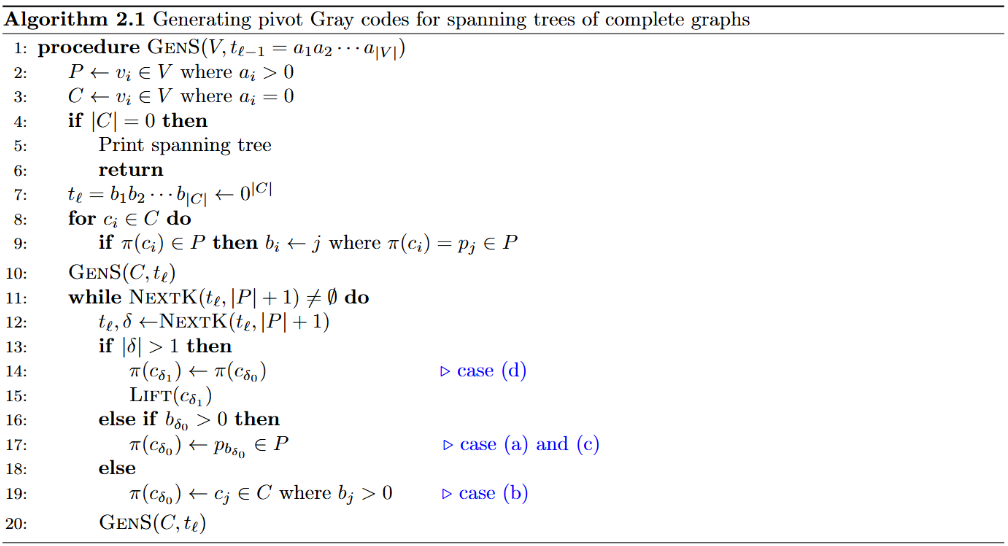
\includegraphics[width=\linewidth]{GenS.png}
        \caption{GenS (Algorithm 2.1)}
    \end{subfigure}
    \hfill
    \begin{subfigure}[b]{0.45\linewidth}
        \centering
        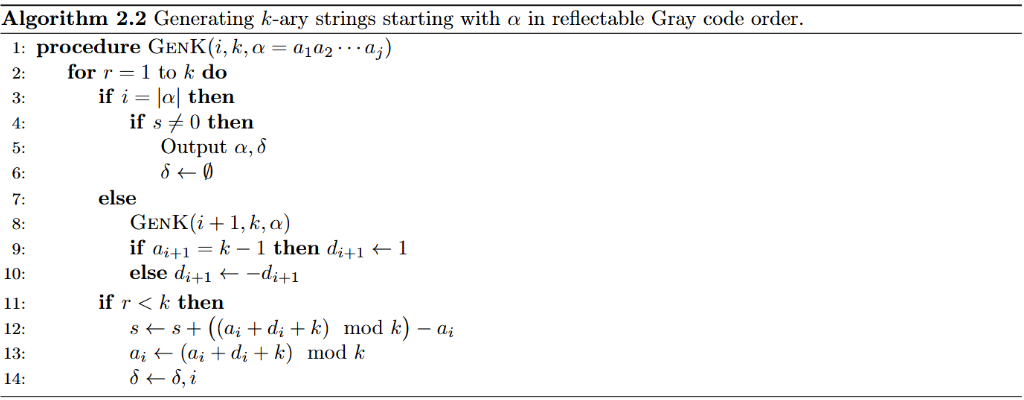
\includegraphics[width=\linewidth]{GenK.png}
        \caption{GenK (Algorithm 2.2)}
    \end{subfigure}
    
    \caption{Algorithms for generating pivot Gray codes for spanning trees of complete graphs.}
    \label{fig:complete_algorithms}
\end{figure}

\begin{figure}[H]
    \centering
    
    \begin{subfigure}[b]{0.32\linewidth}
        \centering
        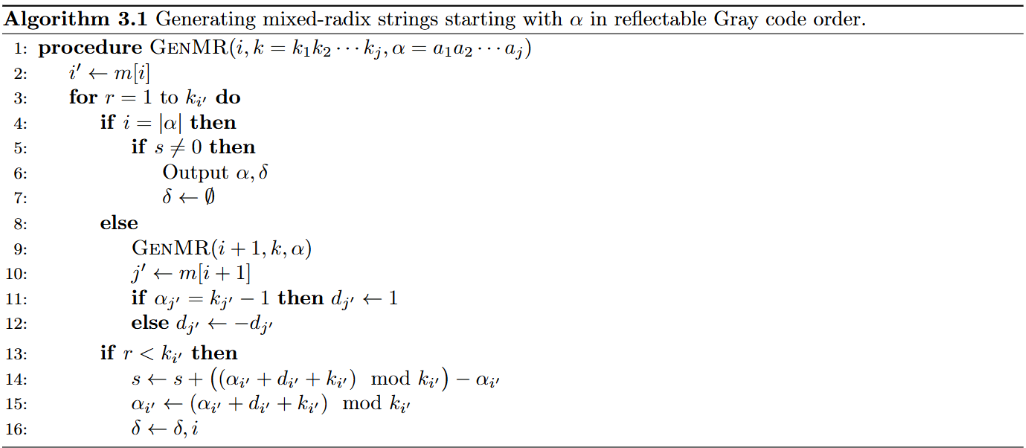
\includegraphics[width=\linewidth]{GenMR.png}
        \caption{GenMR (Algorithm 3.1)}
    \end{subfigure}
    \hfill
    \begin{subfigure}[b]{0.32\linewidth}
        \centering
        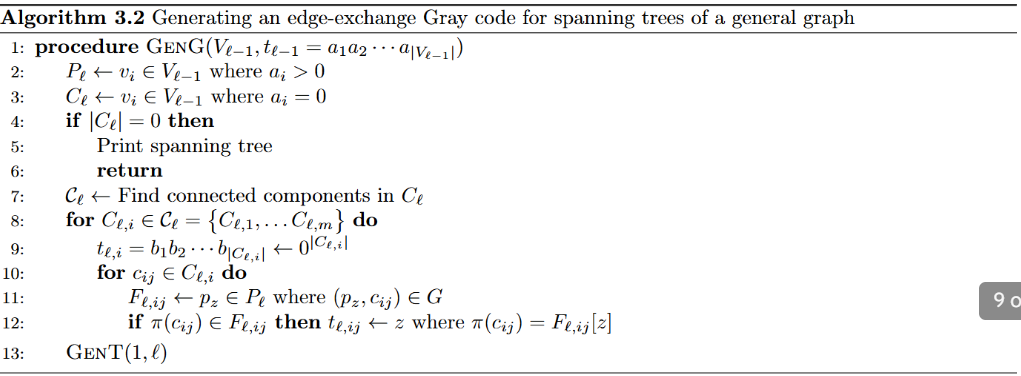
\includegraphics[width=\linewidth]{GenG.png}
        \caption{GenG (Algorithm 3.2)}
    \end{subfigure}
    \hfill
    \begin{subfigure}[b]{0.32\linewidth}
        \centering
        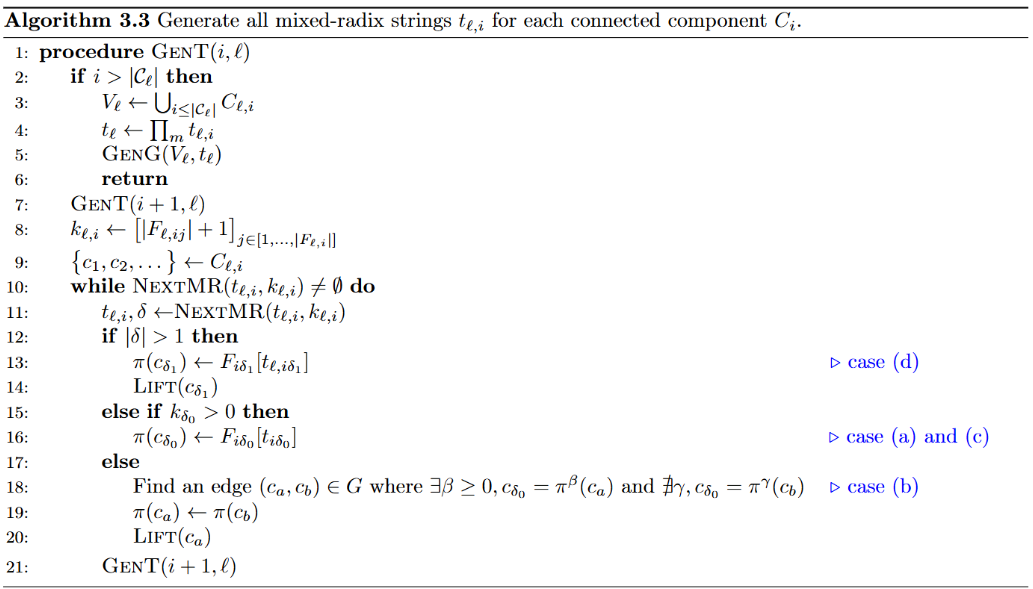
\includegraphics[width=\linewidth]{GenT.png}
        \caption{GenT (Algorithm 3.3)}
    \end{subfigure}
    
    \caption{Algorithms for generating Gray codes for spanning trees of general graphs.}
    \label{fig:general_algorithms}
\end{figure}

\subsection{Description of Input}

The input is a graph $G = (V, E)$, which may be a complete graph $K_n$ or a general connected graph.

\subsection{Desired Output}

The output is a listing of all spanning trees of $G$, generated in Gray code order such that consecutive trees differ by a small edge modification (pivot or edge-exchange).

\subsection{Definitions and Preliminaries}

We introduce several key definitions used throughout this work.

\textbf{Spanning Tree.} A spanning tree of a graph $G$ is a connected, acyclic subgraph that includes all vertices of $G$.

\textbf{Gray Code.} A Gray code is an ordering of combinatorial objects such that consecutive elements differ by a small, local change. In this context, we consider Gray codes for spanning trees, where consecutive trees differ by an edge exchange.

\textbf{Edge-Exchange Gray Code.} An edge-exchange Gray code for spanning trees is a sequence in which each consecutive pair of trees differs by the removal of one edge and the addition of another.

\textbf{Pivot Gray Code.} A pivot Gray code is a stronger form of edge-exchange Gray code in which the removed and added edges share a common vertex. This imposes a stricter locality condition on transitions between consecutive trees.

\textbf{Amortized Time.} An algorithm is said to run in constant amortized time if the average time per operation over a sequence of operations is constant, even if some individual operations may take longer. In this work, we aim to generate each spanning tree in constant amortized time.

\textbf{Complete Graph.} A complete graph $K_n$ is a graph on $n$ vertices in which every pair of distinct vertices is connected by an edge.

\textbf{Mixed-Radix String.} A mixed-radix string is a sequence where each position may have a different base. This is used in the general graph case to represent valid parent assignments for vertices with differing adjacency constraints.

\section{Related Works}
\label{gen_inst}
this part we gotta introduce our reference with a one sentence description of its application to our work, i gotta figure out how to link main.tex to paper.bib

\begin{enumerate}
    \item Nobari, et al.’s longitudinal observational study tracked 20 professional male soccer players for 20 weeks.  found that internal and external load variables are sensitive to factors such as time of season, player positions. TM was measured as mean weekly load / standard deviation of weekly load. TS was measured by weekly load x TM . They used repeated-measures ANOVA and Pearson correlations (\cite{example}).
\end{enumerate}


\section{Motivation}
\subsection{Real World Application}
\label{headings}
Spanning tree enumeration plays an important role across a wide range of scientific fields where alternative network configurations, robustness, and probabilistic behavior must be analyzed. 

One of the earliest motivations for spanning trees arises from electrical network analysis. In electrical systems, Kirchhoff’s laws enable current and voltage analysis by decomposing a network into spanning trees \cite{kirchhoff1847}. Modern work further connects spanning trees to electrical flow optimization, where networks are analyzed through tree-based decompositions \cite{kelner2013electrical, borradaile2020electrical}. Power distribution systems are often operated as radial,tree-like, structures for stability and fault isolation, and enumerating spanning trees allows engineers to explore multiple configurations for power flow while also enabling optimization of energy efficiency, load balancing, and network reconfiguration.

In epidemiology, spanning trees provide a natural representation of transmission pathways, where each tree corresponds to a possible “who-infected-whom” structure during an outbreak. Transmission data is often incomplete or uncertain, so using enumerating spanning trees allows researchers to explore all plausible infection scenarios and perform probabilistic modeling of disease spread \cite{scott2021genomic, rahman2025epidemiology}. This enables better understanding of outbreak dynamics and supports evaluation of intervention strategies such as vaccination and contact tracing. In social network analysis, spanning trees are used to extract simplified backbone structures of complex interaction networks, enabling efficient sampling and analysis of connectivity patterns under structural constraints \cite{lee2020social}.

Spanning trees also play a key role in chemistry and biology by modeling molecular structures and evolutionary relationships. In phylogenetics, spanning trees represent candidate evolutionary trees, allowing researchers to compare competing hypotheses and quantify uncertainty in biological data \cite{graph_theory_mst_applications}. Spanning trees are used in biological sequence analysis, molecular modeling, and studies of network entropy. In physical and technological systems, spanning trees are closely related to models of diffusion, percolation, and connectivity in complex networks. They are also used in the design and analysis of telecommunication systems and in evaluating network complexity and resilience \cite{nature_complex_networks}.

In image processing and computer vision, spanning trees are applied to graph-based representations of images, where pixels are treated as nodes in a graph. Spanning trees enable image segmentation and clustering, grouping pixels into meaningful regions. Enumeration is particularly important in this setting, as different spanning trees correspond to different segmentations, allowing algorithms to explore multiple interpretations of an image and improve robustness \cite{gfg_spanning_tree}. Finally, in network design and reliability, spanning trees represent minimal connectivity structures in communication networks, power grids, and transportation systems. Enumerating spanning trees enables the evaluation of fault tolerance and reliability, since the number and diversity of spanning trees directly reflect the resilience of a network \cite{utdallas_mst, sciencedirect_spanning_tree}.

Across these domains, spanning tree enumeration supports three key objectives: reliability analysis, by quantifying alternative connectivity structures; probabilistic modeling, by exploring all feasible configurations; and optimization, by enabling selection among multiple candidate solutions. These applications highlight the practical importance of efficient spanning tree generation algorithms, such as those developed in this work.

\subsection{Problem Background and Historical Context}

The problem of efficiently enumerating spanning trees has a long history in combinatorics and computer science. For a complete graph $K_n$, Cayley’s formula states that there are $n^{n-2}$ distinct spanning trees, making enumeration exponential in output size. 

The specific problem addressed in our work was posed by Knuth in \textit{The Art of Computer Programming} (Vol. 4A, Section 7.2.1.6, Exercise 101), where he asked whether there exists a \emph{simple revolving-door} method to list all spanning trees of the complete graph $K_n$. In this context, a revolving-door ordering refers to a Gray code, where consecutive spanning trees differ by a small local change, specifically the removal of one edge and the addition of another. Knuth noted that existing approaches, such as Algorithm S, produce such listings but are ``quite complicated'' and lack a clean structure. Knuth’s Algorithm S is hard to understand because it serves more as a starting point to develop an algorithm, providing english version of code for someone else to develop.

%% ADD KNUTHS ALG HERE %%%%
\begin{figure}[H]
    \centering

    % Row 1
    \begin{subfigure}[b]{0.3\linewidth}
        \centering
        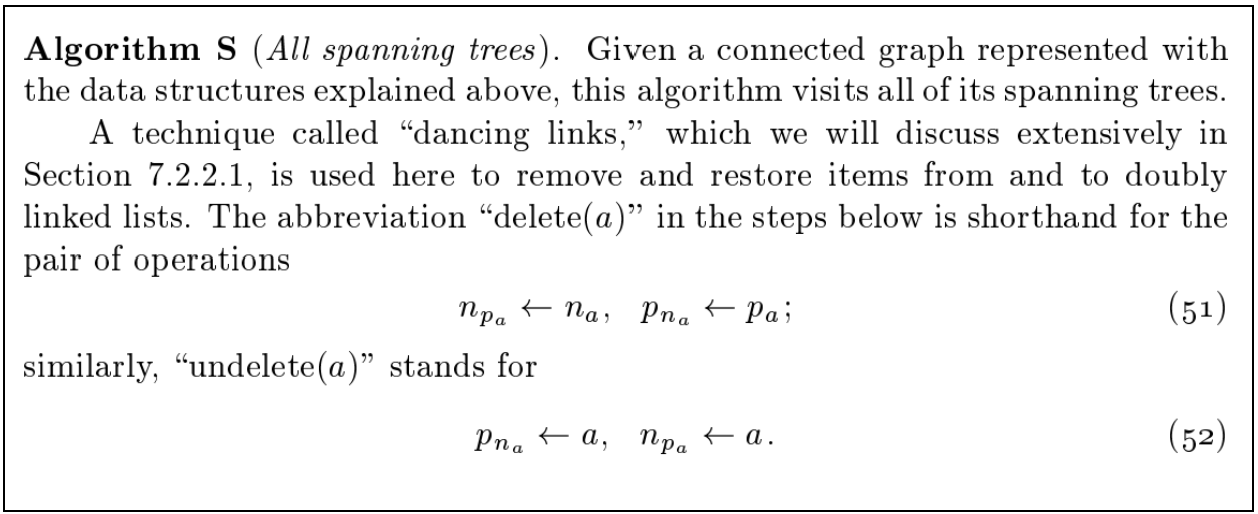
\includegraphics[width=\linewidth]{knuth_1.png}
        \caption{}
    \end{subfigure}
    \hfill
    \begin{subfigure}[b]{0.3\linewidth}
        \centering
        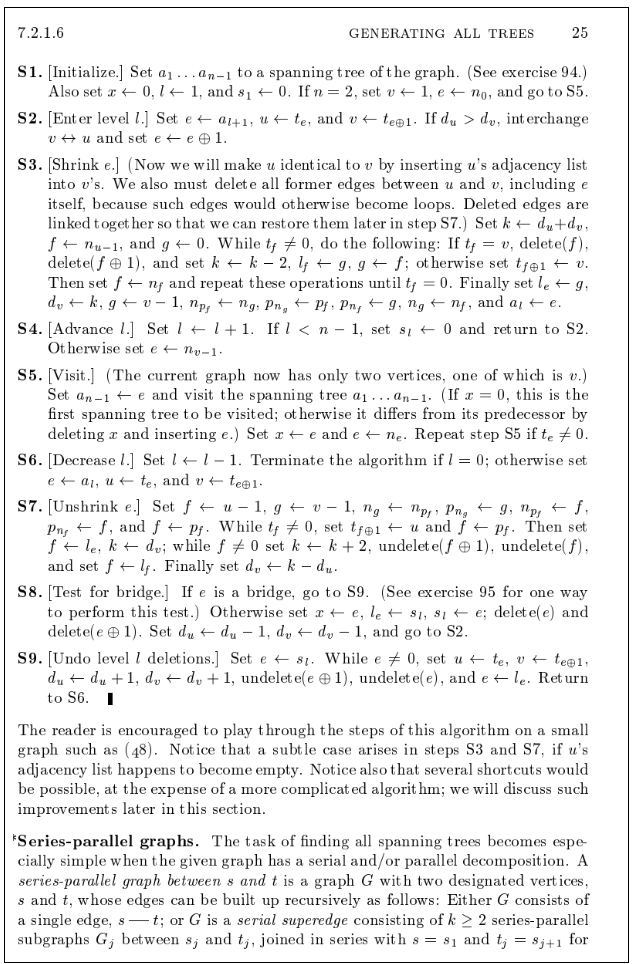
\includegraphics[width=\linewidth]{knuth_2.png}
        \caption{}
    \end{subfigure}
    \hfill
    \begin{subfigure}[b]{0.3\linewidth}
        \centering
        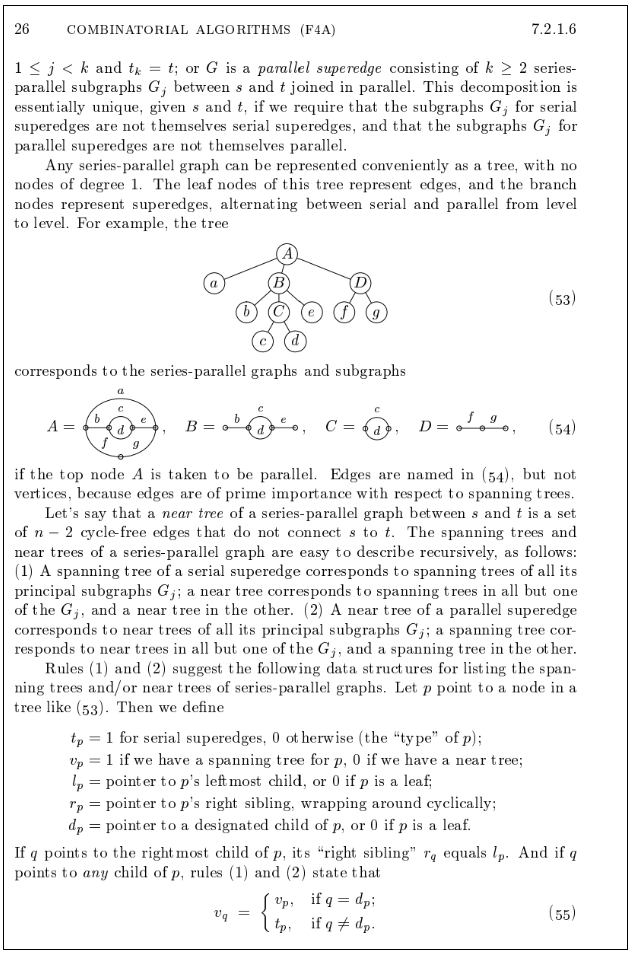
\includegraphics[width=\linewidth]{knuth_3.png}
        \caption{}
    \end{subfigure}

    \vspace{0.5em}

    % Row 2
    \begin{subfigure}[b]{0.3\linewidth}
        \centering
        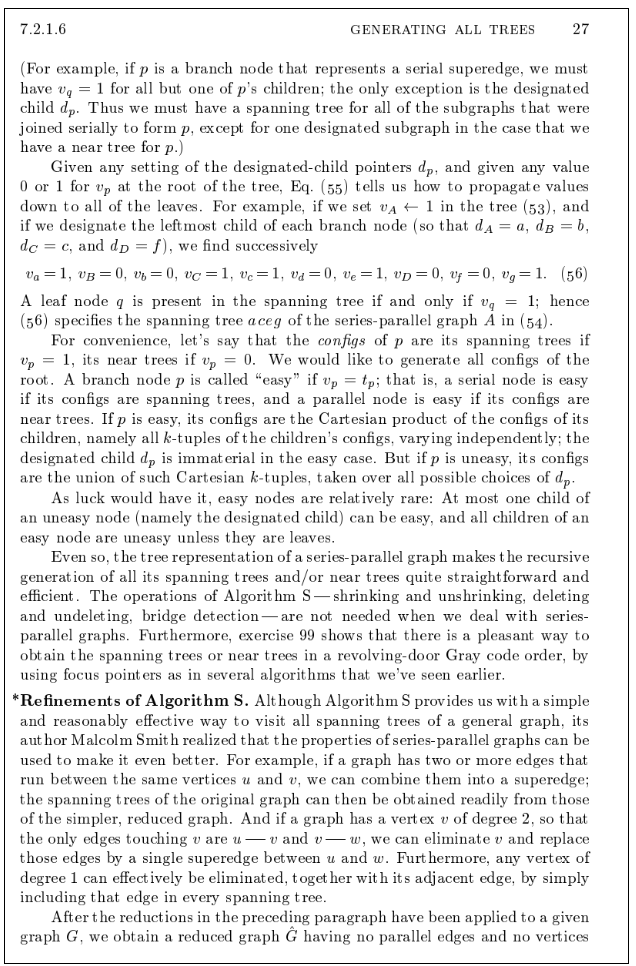
\includegraphics[width=\linewidth]{knuth_4.png}
        \caption{}
    \end{subfigure}
    \hfill
    \begin{subfigure}[b]{0.3\linewidth}
        \centering
        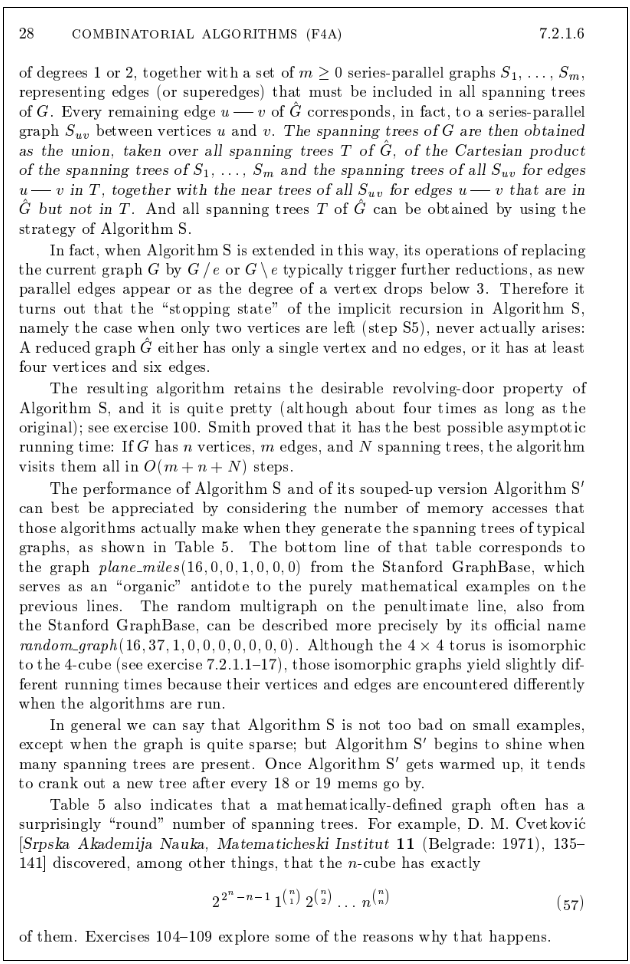
\includegraphics[width=\linewidth]{knuth_5.png}
        \caption{}
    \end{subfigure}
    \hfill
    \begin{subfigure}[b]{0.3\linewidth}
        \centering
        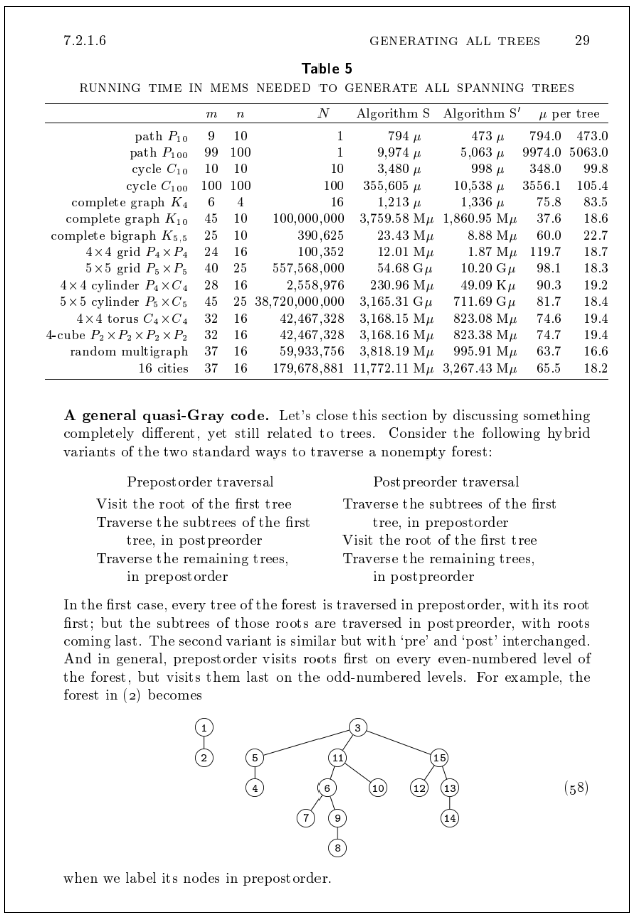
\includegraphics[width=\linewidth]{knuth_6.png}
        \caption{}
    \end{subfigure}

    \caption{Knuth’s Algorithm S and spanning tree enumeration.}
    \label{fig:knuth_algorithms}
\end{figure}

\subsection{Algorithmic Challenges and Contributions}

Designing efficient algorithms for generating spanning trees in Gray code order presents several challenges. First, the number of spanning trees grows exponentially as $n^{n-2}$, which can be lowered by using amortized time. Second, enforcing the Gray code property requires that consecutive spanning trees differ by only a small local modification, which is nontrivial to maintain while ensuring that all trees are generated exactly once. A third challenge arises in imposing stronger constraints of the pivot property, where the removed and added edges must share a common vertex.

From our research we found that these challenges are able to be solved by introducing a novel recursive framework that encodes spanning trees as tuples derived from rooted tree representations. The key idea is to reduce the problem of generating spanning trees to generating Gray codes over structured strings. For complete graphs, this is achieved using $k$-ary Gray codes, while for general graphs, the approach is extended using mixed-radix Gray codes to account for varying adjacency constraints. By mapping changes in these strings to modifications in the corresponding spanning trees, the algorithm ensures that each step corresponds to a valid pivot operation.

The resulting algorithm generates all spanning trees of $K_n$ in pivot Gray code order using constant amortized time per tree and $O(n^2)$ space. Moreover, the framework generalizes to arbitrary connected graphs, producing edge-exchange Gray codes in $O(n^2)$ time. Beyond improving structural simplicity over prior approaches such as Algorithm S, this method also provides proof of Cayley’s formula derived directly from the recursive generation process.

\section{One Algorithm}
\label{others}

Elaborate on one particular algorithm of your choice in more detail.This algorithm does not have to be the current best, it could a previous well-known algorithm or a preliminary/simplified version of recent algorithms. NP-hard problems may admit only approximation algorithms. Do not attempt to explain advanced data structures or mathematical models that go beyond the scope of this project

\subsection{About the Algorithm }

 Explain the main strategy of the algorithm in plain words.

\subsection{pseudo code or code snippets}

we have code snippets for alg 2.1, 2.2, 3.1, 3.2, 3.3

\subsection{analyze runtime}

run time is O(n2).


\section{Implementation}

\subsection{Source and Setup}

The code implementation used in this project was provided from the research paper in python, though the indentation of the code was nonexistent and needed to be fixed. The research paper provided 3 code snippets in python. The first being code to generate pivot Gray codes for spanning trees of complete graphs. The second is to generate an edge-exchange Gray code for spanning trees of a general graph. The third is k\_ary and generates Gray codes for $k$-ary strings and mixed-radix strings. The other two programs utilize k\_ary to enumerate all spanning trees of the user-defined graph and print them out as a parent-pointer list.

The program prompts the user to choose between five different graph types: complete graphs, fan graphs, wheel graphs, the Petersen graph, and custom graphs given by an edge list. For the first three choices, you are prompted for the number of vertices within the graphs. After input, the graph is constructed as an adjacency matrix, the program builds an initial spanning tree using breadth-first search, then begins enumeration. Each spanning tree is outputted in the form of 1->-1; 2->1, 3->2; ..., where every entry gives a vertex and the index of its parent, -1 representing the root. 

The programs only depend on Python's standard library and NumPy, which is utilized to build the adjacency matrix. No other packages are required, which keeps the setup rather minimalist and easy to implement in any Python standard environment. 

\subsection{Testing and Verification}

Testing is focused on two questions: is the correct number of spanning trees produced? Does the Gray code property hold across the output sequence? 

Correctness in regard to the count of spanning trees produced was verified using Cayley's formula that was previously mentioned, which states that a complete graph that has n vertices yields $n^{n-2}$ spanning trees. For n = 4 the expected count to see is 16, and for n = 5 it is 125. The counts with these corresponding n values, for a complete graph, are produced with the algorithm. 

The Gray code property was verified by inspecting the output, by comparing consecutive lines. For each pair of consecutive trees, the parent-pointer strings were compared entry by entry. In each of the cases, exactly one or two entries differed between two consecutive trees. This is consistent with the pivot operation that was described earlier. In which one edge is removed and another is added, sharing a common vertex. In the program output, each spanning tree appeared only once. This confirms that the enumeration visits each spanning tree exactly once. 

\subsection {Recommendations for Readers}

The following notes are intended for readers who wish to run or build on this implementation. 

\begin{itemize}
    \item Python 3.8 or earlier versions is required. The implementation utilizes \texttt{yield from} for recursive generator delegation. Which, is not available for earlier versions of Python.
    \item NumPy is necessary to be installed for all graphs except complete ones. It is used to build the adjacency matrix for the graphs that need it. 
    \item Spanning tree counts grow rather rapidly as the number of vertices increases; this is more apparent for complete graphs. Cayley's formula gives a count of $n^{n-2}$ spanning trees, for complete graphs, which reaches a count over one million at n = 8 and over one billion at n = 11. (NEED TO CONTINUE HERE I AM TOO TIRED)
\end{itemize}


\section{Conclusion}



\section{References}


Cite all resources used for preparing the project report (including books, papers, urls, and Artificial Intelligence). Add reference for every claim that is not substantiated within the project report. Add references and pointers to related topics that you find interesting but go beyond the scope of the project. Text or code taken from any source must be clearly indicated with quotation marks, with a clear reference to the source.

\bibliography{paper}


%%%%%%%%%%%%%%%%%%%%%%%%%%%%%%%%%%%%%%%%%%%%%%%%%%%%%%%%%%%%

\appendix

\section{Credits}


All members participated in team meetings, research, and presentation preparation. Individual writing contributions are as follows: Zachary wrote sections 1 and 3 which include the Problem and Motivation section, including the formal problem definition, Knuth's open problem background, and real-world applications of spanning tree enumeration. Richard wrote the History section, covering the development of spanning tree enumeration from early algorithms through Gray codes, the revolving-door problem, the progression to pivot Gray codes leading to this paper's contribution and compiled all references and credits. Behrouz wrote the One Algorithm section, providing a detailed explanation of the GenS algorithm including the tuple encoding, the four pivot-change cases from Lemma 2.2, pseudocode walkthrough, and running time analysis. Marcus wrote the Implementation section, including testing of the provided Python code, verification of tree counts against Cayley's formula, reader recommendations for using the code.


\end{document}